%%%%%%%%%%%%%%%%%%%%%%%%%%%%%%%%%%%%%%%%%%%%%%%%%%%%%%%%%%%%%%%%%%%%%%%%%%%%%%%%
%%%%%%%%%%%%%%%%%%%%%%%%%%%%%%%%%%%%%%%%%%%%%%%%%%%%%%%%%%%%%%%%%%%%%%%%%%%%%%%%
%%                          AUTHOR: BIBEKANANDA DATTA                         %%
%%                             (C) SEPTEMBER 2023                             %%
%%                      PhD STUDENT, MECHANICAL ENGINEERING                   %%
%%                           JOHNS HOPKINS UNIVERSITY                         %%
%%%%%%%%%%%%%%%%%%%%%%%%%%%%%%%%%%%%%%%%%%%%%%%%%%%%%%%%%%%%%%%%%%%%%%%%%%%%%%%%
%%%%%%%%%%%%%%%%%%%%%%%%%%%%%%%%%%%%%%%%%%%%%%%%%%%%%%%%%%%%%%%%%%%%%%%%%%%%%%%%
%%             PLEASE CHECK THE README.md FILE BEFORE YOU PROCEED             %%
%%              it may be convenient to read this file on GitHub              %%
% https://github.com/bibekananda-datta/JH-MechE-Dissertation-Proposal-Template %
%% template hosted on the GitHub repository is likely to be the most updated  %%
%%%%%%%%%%%%%%%%%%%%%%%%%%%%%%%%%%%%%%%%%%%%%%%%%%%%%%%%%%%%%%%%%%%%%%%%%%%%%%%%


%%%%%%%%%%%%%%%%%%%%%%%%%%%%%%%%%%%%%%%%%%%%%%%%%%%%%%%%%%%%%%%%%%%%%%%%%%%%%%%%
% this is an unofficial template for the thesis or dissertation proposal in 
% the Department of Mechanical Engineering at Johns Hopkins University. 
% consult with the department or advisor before using the template.
% this template includes comments on the department-suggested page limits. 
% however, it is the user's responsibility to ensure the formatting conforms 
% with the advisor or proposal committee or department's requirement.
% this template is based on the LaTeX article class and uses BibLaTeX as 
% bibliographic manager. Use a citation manager to generate the BibLaTeX file.
%%%%%%%%%%%%%%%%%%%%%%%%%%%%%%%%%%%%%%%%%%%%%%%%%%%%%%%%%%%%%%%%%%%%%%%%%%%%%%%%



%%%%%%%%%%%%%%%%%%%%%%%%%%%%%%%%%%%%%%%%%%%%%%%%%%%%%%%%%%%%%%%%%%%%%%%%%%%%%%%%
%% if possible, please make your formatting changes here through the variables 
%% go through all the variables and understand what role they play in formatting
%%%%%%%%%%%%%%%%%%%%%% LIST OF VARIABLES FOR FORMATTING %%%%%%%%%%%%%%%%%%%%%%%%

\def\FontPackage{lmodern}                   % latin modern font (you can also change it to times)
\def\BibFileName{references.bib}            % name of BibLaTeX file with all the bibliography

\def\NoSectionLevel{3}                      % 3 levels for sections ... to subsubsection
\def\TocIndent{0}                           % indentation in the list of figs and tables
\def\NoTocLevel{3}                          % no of levels showed in the table of contents
%% 3 levels mean section to subsubsection.. decrease if you want less to show in TOC

\def\GlobalMargin{1.0in}                    % margin on all sides

%%%% font size and typeset for different environments
%% check here for details: https://en.wikibooks.org/wiki/LaTeX/Fonts
\def\BaseFont{12pt}
\def\TitleFont{\large\bfseries\MakeUppercase}
\def\SectionFont{\large\bfseries}           % section heading font format
\def\SubsectionFont{\normalsize\bfseries}   % subsection heading font format
\def\SubsubsectionFont{\normalsize\itshape} % subsubsection heading font format
\def\CaptionFontSize{small}                 % caption font size
\def\CaptionFontType{bf}                    % boldface label for captions
\def\CaptionSeparator{colon}                % separates caption heading from text. can use 'period' as well

\def\TitlePageSpacing{\singlespacing}       % spacing of the title page contents
\def\MainTextSpacing{\singlespacing}        % double spacing in the main text (JH library requirement)
\def\TOCTextSpacing{\onehalfspacing}        % one-half spacing for TOC texts
\def\ParagraphSpacing{\baselineskip}        % spacing between paragraph
\def\ParagraphIndent{0}                     % indentation at the beginning of the paragraph
\def\FullCiteSpacing{1.0}                   % spacing in a fullcite item
\def\LOTItemSpacing{3.5 pt}                 % spacing between LOT/LOF items
\def\BibItemSpacing{0.4\baselineskip}       % spacing between bibliographic items in reference
\def\FootnoteSpacing{0.5\baselineskip}      % spacing between footnotes
\def\CaptionSpacing{0}                      % spacing between the figure and the caption (unit: pt)

\def\GlobalTableSpacing{1.0}                % global spacing parameter for table
%% if this seems too widespread for you, try changing it locally using
%% \begin{group} ... \renewcommand{\arraystretch} ... \end{group} commands

%%%%%%%%%%%%%%%%%%%% END LIST OF VARIABLES FOR FORMATTING %%%%%%%%%%%%%%%%%%%%%%




%%%%%%%%%%%%%%%%%%%%%%%%%%%%%%%%%%%%%%%%%%%%%%%%%%%%%%%%%%%%%%%%%%%%%%%%%%%%%%%%
%% add packages as needed but sometimes the order of the packages matters.
%% I primarily tried to load the packages in alphabetical order or based on
%% their functionalities (all math/ table packages) unless there is an issue
%% with package dependency, so I included packages in that order. remember,
%% you may get warnings/ errors for the order in which packages are included
%% you may have to change the options in biblatex package for the bibliography
%%%%%%%%%%%%%%%%%%%%%%%%%%% LaTeX CLASS AND PACKAGES %%%%%%%%%%%%%%%%%%%%%%%%%%%

\documentclass[\BaseFont,letterpaper]{article} % document class (article w/ 12 pt)

\usepackage[utf8]{inputenc}	                % for encoding input character
\usepackage[pagewise,mathlines]{lineno}     % linenumbers


%% math packages
\usepackage{amsfonts,amssymb,amsmath,amsthm,autobreak,cancel,dsfont,mathtools,mathbbol,mathrsfs,siunitx,upgreek}

\usepackage[ruled]{algorithm2e}             % to manage algorithm environment
\usepackage[titletoc]{appendix}             % to manage appendix chapters
\usepackage[american]{babel}                % for different language typography

%% bibliographic package (make sure your bib file is in BibLaTeX format)
%% use Zotero or some other reference manager to generate the BibLaTeX file
%% change the style or other options if you need to
\usepackage[backend=biber, defernumbers=true, style=nature, maxnames=9, date=year, isbn=false, url=false, doi=true]{biblatex}
% \usepackage[backend=biber, defernumbers=true, style=apa, isbn=false, url=false, doi=true]{biblatex}

\usepackage{blindtext}                      % to generate random filler texts
\usepackage{calc}                           % to set arithmetic arguments for spacing
\usepackage{caption}                        % to manage captions
\usepackage{color}                          % color related packages
\usepackage{csquotes,epigraph,varwidth}     % for managing quotes
\usepackage{enumitem}                       % to manage list environment
\usepackage{float}                          % to manage floating environment
\usepackage[T1]{fontenc}                    % for font encoding
\usepackage[bottom]{footmisc}               % footnote environment management
\usepackage{graphicx,wrapfig}               % to manage images
\usepackage{geometry}                       % to manage margins and others
\usepackage{fancyhdr}                       % for header/ footer settings
\usepackage[dvipsnames]{xcolor}
\usepackage[a-1b]{pdfx}                     % to generate PDF/A file (before hyperref)
\usepackage[pdfa]{hyperref}                 % for hyperlinks
\usepackage[all]{hypcap}                    % for captions on the side of figures
\usepackage{ifthen}                         % if-then statement in algorithm
\usepackage{lscape}                         % landscape mode
\usepackage{listings}                       % to include codes

%% table related packages
\usepackage{booktabs,longtable,makecell,multicol,multirow,tabularx,xltabular}

\usepackage{tocloft}                        % to manage table of contents
\usepackage{parskip}                        % paragraph spacing 
\usepackage{setspace}                       % sets space between lines
\usepackage{seqsplit}                       % splits long character sequence
\usepackage[rightcaption]{sidecap}          % for sideway captions
\usepackage{titlesec}                       % managing different titles
\usepackage[absolute]{textpos}              % to position text
\usepackage{tikz}                           % package for drawing
\usepackage{subcaption}                     % individual panel and caption

%% add more packages and options as you need

%%%%%%%%%%%%%%%%%%%%%%%%% END LaTeX CLASS AND PACKAGES %%%%%%%%%%%%%%%%%%%%%%%%%



%%%%%%%%%%%%%%%%%%%%%%%%%%%%% DOCUMENT FORMATTING %%%%%%%%%%%%%%%%%%%%%%%%%%%%%%

%%% choice a font form (or add something else) for your thesis (uncomment one option)
\usepackage{\FontPackage}       
% if you want to use Palatino font, use the following and comment above line
% \usepackage[sc]{mathpazo}                  % palatino font family

%%% I use Zotero to generate the BibLaTeX file and include it in the same directory
\addbibresource{\BibFileName}

%%% margin settings with geometry package
\geometry{margin=\GlobalMargin, nomarginpar}

%%% settings for the hyperref package
\hypersetup{linktocpage, unicode, linktoc=all, colorlinks=true, citecolor=blue, filecolor=blue, linkcolor=blue, urlcolor=blue}
\urlstyle{rm}   % to remove the default URL style (tt format)

%%% settings for figure caption
\captionsetup{belowskip=\CaptionSpacing pt, font=\CaptionFontSize, labelfont=\CaptionFontType, labelsep=\CaptionSeparator, hypcap=true} 

\setcounter{tocdepth}{\NoTocLevel}                      % list depth in ToC

\renewcommand{\cfttoctitlefont}{\SectionFont}           % font for ToC title
\renewcommand{\cftloftitlefont}{\SectionFont}           % font for LoF title
\renewcommand{\cftlottitlefont}{\SectionFont}           % font for LoT title

\setlength{\cftbeforesecskip}{0.5\baselineskip}         % space between sections in TOC
\renewcommand{\cftsecleader}{\cftdotfill{\cftdotsep}}   % dots for sections too

% tweak to LoF/ LoT to add 'Figure' & 'Table' to the figure and table caption listing
% to change the distance to the start of the figure/ table title
\setlength{\cftfigindent}{\TocIndent pt}                % indentation from figures in LoF
\renewcommand{\cftfigpresnum}{\bfseries Figure }
\setlength{\cftfignumwidth}{\widthof{\textbf{Figure~99.999~}}}
\setlength{\cftbeforetabskip}{\LOTItemSpacing}          % spacing between each item
%
\setlength{\cfttabindent}{\TocIndent pt}                % indentation from tables in LoT
\renewcommand{\cfttabpresnum}{\bfseries Table }
\setlength{\cfttabnumwidth}{\widthof{\textbf{Table~99.100~}}}
\setlength{\cftbeforefigskip}{\LOTItemSpacing}          % spacing between each item


%%%% font and style for the section, subsection, subsubsection, etc.
\setcounter{secnumdepth}{\NoSectionLevel}   % section to ... subsubsection ...
\titleformat{\section}{\SectionFont}{\thesection}{1em}{}[{\titlerule}]
\titleformat*{\subsection}{\SubsectionFont}
\titleformat*{\subsubsection}{\SubsubsectionFont}
%% delete [{\titlerule}] to remove all the underlines below the section title


%%%% paragraph, footnote, bib item, and table spacing
\setlength{\parskip}{\ParagraphSpacing}     % paragraph spacing
\setlength{\parindent}{\ParagraphIndent pt} % paragraph indentation
\setlength{\footnotesep}{\FootnoteSpacing}  % footnote separation
\setlength{\bibitemsep}{\BibItemSpacing}    % bib item separation 
\def\arraystretch{\GlobalTableSpacing}      % spacing in table

%%%% settings for math environment
\allowdisplaybreaks[1]                      % page break in math formula
\numberwithin{equation}{section}            % eqn no begins with section no
\setcounter{MaxMatrixCols}{20}              % maximum columns in matrix = 20


%%% settings for bibliography
\AtBeginBibliography{\urlstyle{rm}}
\DeclareFieldFormat{titlecase}{\MakeSentenceCase*{#1}}

\DeclareBibliographyCategory{mypapers}
\newcommand{\mybibexclude}[1]{\addtocategory{mypapers}{#1}}

%% settings for TikZ library (add more if you need them)
\usetikzlibrary{decorations.pathreplacing, positioning, arrows.meta, shapes,}


%%%%%%%%%%%%%%%%%%%%%%%%%%% END DOCUMENT FORMATTING %%%%%%%%%%%%%%%%%%%%%%%%%%%




%%%%%%%%%%%%%%%%%%%%%%%%%%%%%%%%%%%%%%%%%%%%%%%%%%%%%%%%%%%%%%%%%%%%%%%%%%%%%%%
%% add all your custom math settings and macros in the following section.
%% this is where LaTeX supremacy becomes a thing. you can customize a lot.
%%%%%%%%%%%%%%%%%%%%%%%%%%%%%% MATH MACROS %%%%%%%%%%%%%%%%%%%%%%%%%%%%%%%%%%%%

%%% Define math symbols and macros
\newcommand{\dC}{$^{\circ}$C}           % degree celsius symbol
\newcommand{\vect}[1]{\mathbf{#1}}      % boldface for vectors and tensors
\DeclareMathOperator{\T}{{\top}}        % transpose of a matrix/ tensor
\DeclareMathOperator{\tr}{tr}           % trace of a matrix
\DeclareMathOperator{\divg}{div}        % divergence of vector and tensor
\DeclareMathOperator{\grad}{grad}       % gradient of vector and tensor
\DeclareMathOperator{\curl}{curl}       % curl of vector and tensor

%% these are just some examples; add more macros for your custom symbols

%%%%%%%%%%%%%%%%%%%%%%%%%%%%% END MATH MACROS %%%%%%%%%%%%%%%%%%%%%%%%%%%%%%%%%


%%%%%%%%%%%%%%%%%%%%%%%%%%%%%%%%%%%%%%%%%%%%%%%%%%%%%%%%%%%%%%%%%%%%%%%%%%%%%%%
%% add all your non-mathematical macros and other random settings here.
%%%%%%%%%%%%%%%%%%%%%%%%%%%%%% OTHER MACROS %%%%%%%%%%%%%%%%%%%%%%%%%%%%%%%%%%%

\newcommand{\COMMENT}{\textcolor{red}}
\newcommand{\ADDCITATION}{\COMMENT{(ADD CITATION)}}

%% you can also add more simple comments here as you need
%% you can use some other packages for more complicated review and comment section

%%% to add small quotes
\newcommand{\say}[2]{\hfill\small\enquote{\textit{#1}}{ - \small\textsc{#2}.}}

%%%%%%%%%%%%%%%%%%%%%%%%%%%% END OTHER MACROS %%%%%%%%%%%%%%%%%%%%%%%%%%%%%%%%%
%%%%%%%%%%%%%%%%%%%%%%%%%%%%%%%%%%%%%%%%%%%%%%%%%%%%%%%%%%%%%%%%%%%%%%%%%%%%%%%

% \usepackage[color=red,unit=in,type=upperleft,showframe]{fgruler}

%%%%%%%%%%%%%%%%%%%%%%%%%%%%%%%%%%%%%%%%%%%%%%%%%%%%%%%%%%%%%%%%%%%%%%%%
%%%%%%%%%%%%%%%%%%%%%%%%%%%% BEGIN DOCUMENT %%%%%%%%%%%%%%%%%%%%%%%%%%%%

\begin{document}

% \linenumbers                      % may find it useful during drafting
%% place the command wherever you want to start numbering the line


%%%%%%%%%%%%%%%%%%%%%%%%%%%%%%%%%%%%%%%%%%%%%%%%%%%%%%%%%%%%%%%%%%%%%%%%
%%%%%%%%%%%%%%%%%%%%%%%%%%% BEGIN TITLE PAGE %%%%%%%%%%%%%%%%%%%%%%%%%%%

%%%%%%%%%%%%%%%%%%%%%%%%%%% TITLE AND AUTHOR %%%%%%%%%%%%%%%%%%%%%%%%%%%
\TitlePageSpacing \thispagestyle{empty}

\begin{center}
    Doctoral dissertation proposal submitted to the \\
    Department of Mechanical Engineering of The Johns Hopkins University
    
    \vspace{0.5in}                      % space between statement and title
    {\TitleFont {A simple \LaTeX\ template for MechE dissertation proposal at Johns Hopkins University} \par}  
    %% tentative thesis title (\par is needed for proper spacing)
    
    \vspace{0.25in}                     % space between title and author
    
    Author Name                         % author name (student)
\end{center}
%%%%%%%%%%%%%%%%%%%%%%%%% END TITLE AND AUTHOR %%%%%%%%%%%%%%%%%%%%%%%%%


%%%%%%%%%%%%%%%%%%%%%%%%%%%% COMMITTEE MEMBERS %%%%%%%%%%%%%%%%%%%%%%%%%
%% if you have multiple advisors/co-advisors, you can add them side-by-side
%% like the committee members as shown below using the 'minipage' environment
%% adjust the space in \vspace{ } command if you want to fit more members
%% you can also condense information for each advisor/ member to make space

\vspace{0.75in}                         % space between author and advisor
\begin{center}
    \textbf{Primary advisor}
    
    Dr. Chuck Darwin \\
    Professor \\
    Department of Mechanical Engineering \\
    Johns Hopkins University, Baltimore, MD
\end{center}

\vspace{0.35in}
\centerline{\textbf{Dissertation proposal committee members}}

\begin{minipage}[t]{0.5\textwidth}
	\begin{flushleft}
	Dr. Albrecht Einstein \\
    Professor \\
    Department of Mechanical Engineering \\
    Johns Hopkins University, Baltimore, MD
	\end{flushleft}
\end{minipage}
~
\begin{minipage}[t]{0.5\textwidth}
	\begin{flushleft}
    Dr. Stewart Hawking \\
    Professor \\
    Department of Mechanical Engineering \\
    Johns Hopkins University, Baltimore, MD 
	\end{flushleft}
\end{minipage}
\vspace{0.75in}                     % space between committee members and location

%%%%%%%%%%%%%%%%%%%%%%%%%% END COMMITTEE MEMBERS %%%%%%%%%%%%%%%%%%%%%%%

%%%%%%%%%%%%%%%%%%%%%%%%%%% TIME AND LOCATION %%%%%%%%%%%%%%%%%%%%%%%%%%
\begin{center}
    Baltimore, Maryland \\          % location 
    Month YEAR                      % like May 2024 (month and year of submission)
    
    %%%% copyright statement is optional (but this will protect your ideas)
    %% this is placed 1.5 inches above the bottom of the page
    {\begin{textblock*}{\textwidth}(\GlobalMargin,9.5in)
        \copyright\ YEAR Author Name. All rights reserved.
    \end{textblock*}
    \null}
\end{center}

%%%%%%%%%%%%%%%%%%%%%%%%% END TIME AND LOCATION %%%%%%%%%%%%%%%%%%%%%%%%

%%%%%%%%%%%%%%%%%%%%%%%%%%%% END TITLE PAGE %%%%%%%%%%%%%%%%%%%%%%%%%%%%
%%%%%%%%%%%%%%%%%%%%%%%%%%%%%%%%%%%%%%%%%%%%%%%%%%%%%%%%%%%%%%%%%%%%%%%%



%%%%%%%%%%%%%%%%%%%%%%%%%%%%%%%%%%%%%%%%%%%%%%%%%%%%%%%%%%%%%%%%%%%%%%%%
%%%%%%%%%%%%%%%%%%%%%%%%%%%%% FRONT MATTER %%%%%%%%%%%%%%%%%%%%%%%%%%%%%
%%%%%%%%%%%%%%%%%%%%%%%%%%%%% BEGIN ABSTRACT %%%%%%%%%%%%%%%%%%%%%%%%%%%

\clearpage 
\pagenumbering{roman}
\setcounter{page}{2}
\MainTextSpacing
\addcontentsline{toc}{section}{Abstract}
\section*{Abstract}

%%% write your abstract and keywords here
\blindtext

%%%%%%%%%%%%%%%%%%%%%%%%%%%%%% END ABSTRACT %%%%%%%%%%%%%%%%%%%%%%%%%%%%

%%%%%%%%%%%%%%%%%%%%%%%%%%%%%%%%% LISTS %%%%%%%%%%%%%%%%%%%%%%%%%%%%%%%%

%% single spacing appears to be too cramped and double spacing is too relaxed
{
\clearpage
\TOCTextSpacing                         % one-half spacing for the TOC
\hypersetup{linkcolor=black}            % local hyperref settings to make the TOC appear black (you can comment it out if you would like the default)
\renewcommand{\contentsname}{Table of Contents \vspace{3.5pt} \hrule}
\tableofcontents


\clearpage \phantomsection
\addcontentsline{toc}{section}{List of Tables}
\renewcommand{\listtablename}{List of Tables \vspace{3.5pt} \hrule}
\listoftables


\clearpage \phantomsection
\addcontentsline{toc}{section}{List of Figures}
\renewcommand{\listfigurename}{List of Figures \vspace{3.5pt} \hrule}
\listoffigures
}

%% delete \vspace{3.5pt} \hrule if you want to remove the underlines

%%%%%%%%%%%%%%%%%%%%%%%%%%%%%%% END LISTS %%%%%%%%%%%%%%%%%%%%%%%%%%%%%%
%%%%%%%%%%%%%%%%%%%%%%%%%%% END FRONT MATTER %%%%%%%%%%%%%%%%%%%%%%%%%%%
%%%%%%%%%%%%%%%%%%%%%%%%%%%%%%%%%%%%%%%%%%%%%%%%%%%%%%%%%%%%%%%%%%%%%%%%


%%%%%%%%%%%%%%%%%%%%%%%%%%%%%%%%%%%%%%%%%%%%%%%%%%%%%%%%%%%%%%%%%%%%%%%%
%%%%%%%%%%%%%%%%%%%%%%%%%%% BEGIN MAIN TEXT %%%%%%%%%%%%%%%%%%%%%%%%%%%%

\clearpage \MainTextSpacing \pagenumbering{arabic}

%%%%%%%%%%%%%%%%%%%%%%%%%%%%%% BACKGROUND %%%%%%%%%%%%%%%%%%%%%%%%%%%%%%

\section{Background and significance}           %%% 2 page limit 

\blindtext \cite{dirac}.

\begin{figure}[ht]
\begin{center}
    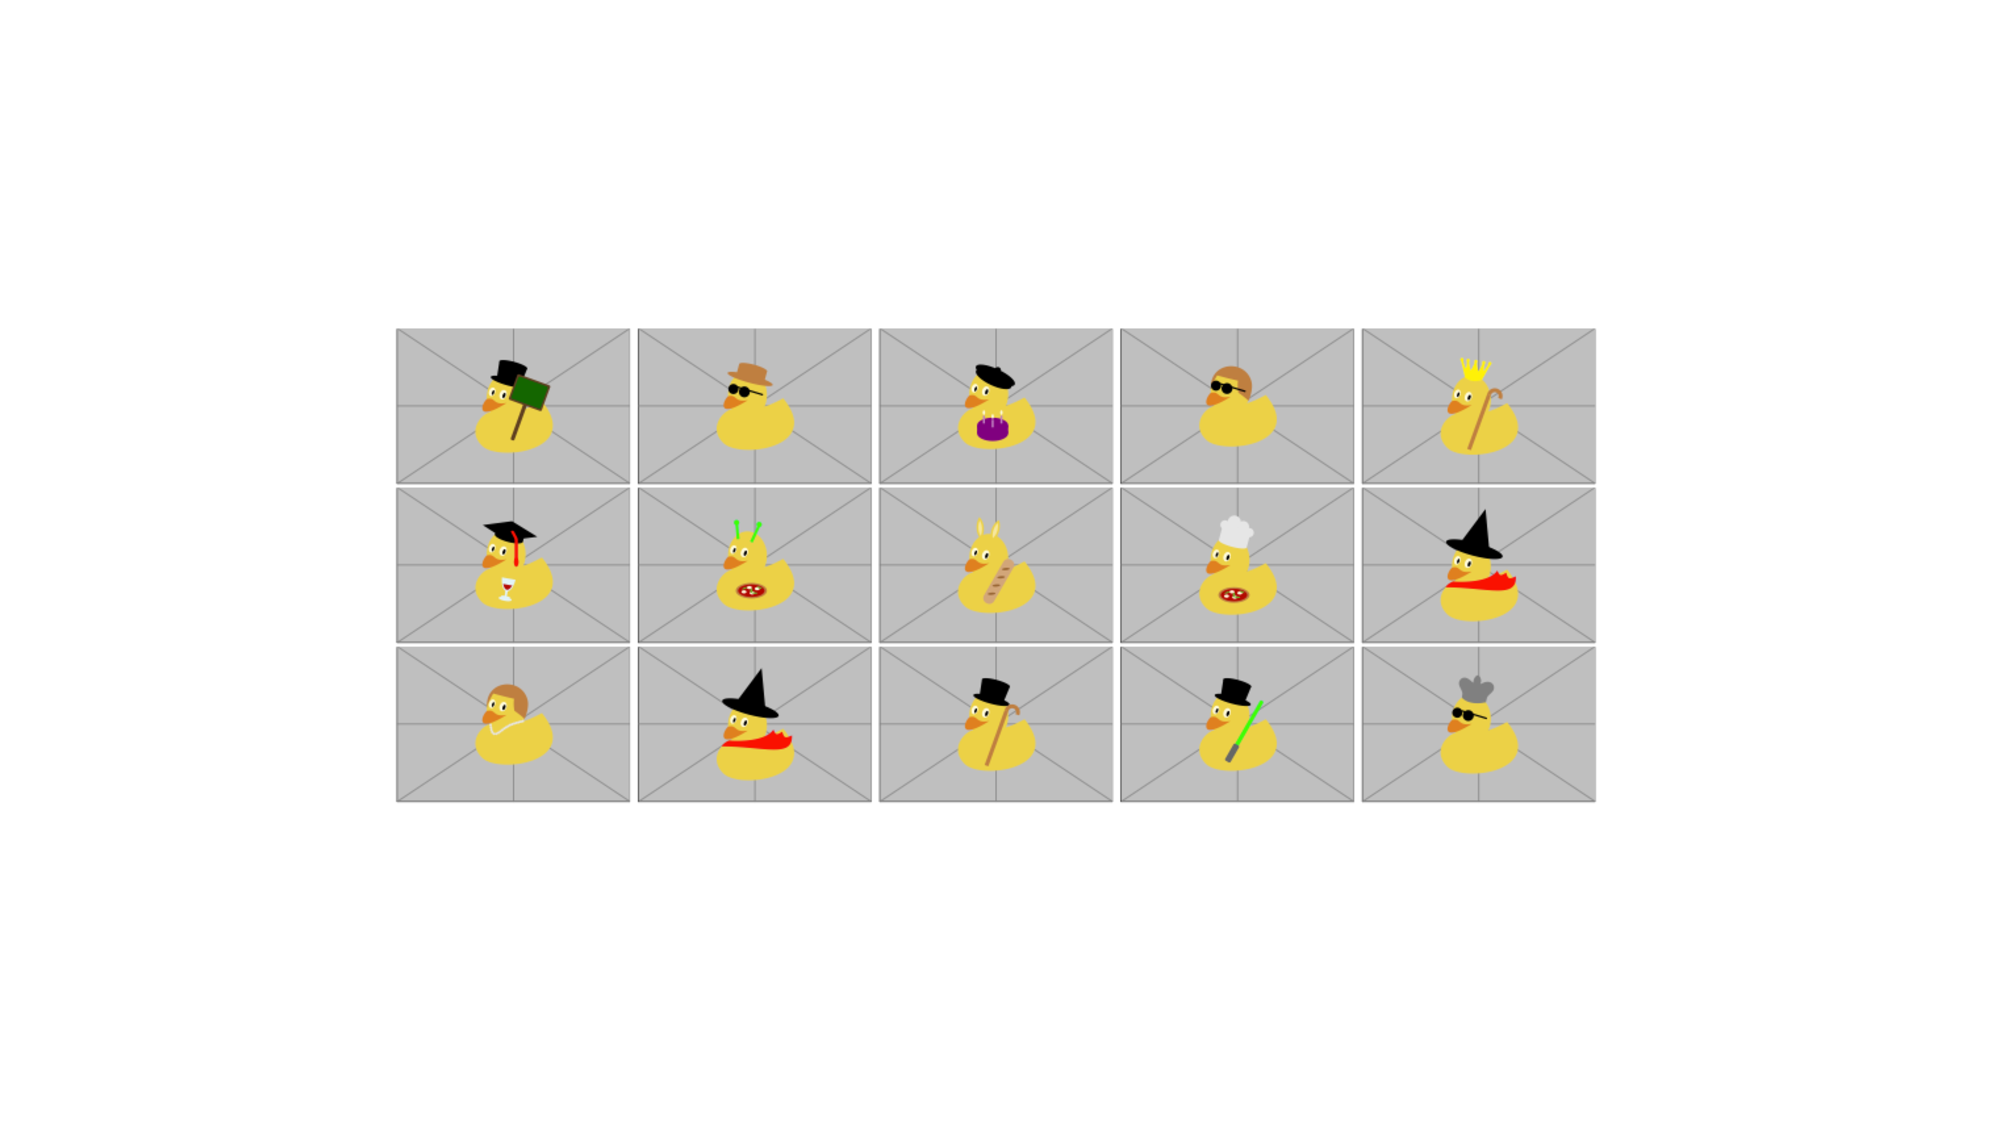
\includegraphics[width=\textwidth, trim={6cm 5cm 6cm 5cm},clip,page=1] {figures.pdf}
    \caption{Here are some photos of ducks to make you feel happy in tough times.}
    \label{fig:ducks}
\end{center}
\end{figure}


%%%%%%%%%%%%%%%%%%%%%%%%%%%%%%%%%%%%%%%%%%%%%%%%%%%%%%%%%%%%%%%%%%%%%%%%%
%% for subsections and subsubsection, I didn't particularly like having 
%% numbered environments because they appeared confusing with my objectives  
%% and task numbering. so I used unnumbered subsections and subsubsections 
%% and added these env. to the table of contents using \phantomsection and 
%% \addcontentsline commands before and after the corresponding environment.
%%%%%%%%%%%%%%%%%%%%%%%%% RESEARCH OBJECTIVES %%%%%%%%%%%%%%%%%%%%%%%%%%%

\section{Research objectives}                   %%% suggested: 1 page limit

\blindtext \cite{knuthwebsite}

%% 
\phantomsection
\subsection*{Objective 1: Some major objective here}
\addcontentsline{toc}{subsection}{Objective 1: Some major objective here}

\blindtext

%% add more objectives (one objective is not enough you know it)





%%%%%%%%%%%%%%%%%%%%%%%%%%%%%%%%%%%%%%%%%%%%%%%%%%%%%%%%%%%%%%%%%%%%%%%%%
%% I used unnumbered subsections and subsubsections in this section as well
%% and added these env. to the table of contents using \phantomsection and 
%% \addcontentsline commands before and after the corresponding environment.
%%%%%%%%%%%%%%%%%%%%%%% METHODOLOGY AND RESULTS %%%%%%%%%%%%%%%%%%%%%%%%%

\section{Proposed methodology and results}      %%% suggested: 4 page limit

\blindtext

\subsection{Task 1: Major project task heading here related to objective 1}

\blindtext


\phantomsection
\subsubsection*{Subtask 1.1: Some sub-task here}
\addcontentsline{toc}{subsubsection}{Subtask 1.1: Some sub-task here}

\blindtext

\begin{table}[ht]
\centering
\begin{tabular}{c c c c} 
\toprule \toprule
Col1 & Col2 & Col2 & Col3 \\ 
\toprule \toprule
1 & 6 & 87837 & 787 \\ 
2 & 7 & 78 & 5415 \\
3 & 545 & 778 & 7507 \\
4 & 545 & 18744 & 7560 \\
5 & 88 & 788 & 6344 \\ 
\bottomrule
\end{tabular}
\caption{Table to test captions and labels taken from Overleaf.}
\label{table:1}
\end{table}


\subsubsection*{Subtask 1.2: Some other sub-task here}
\addcontentsline{toc}{subsubsection}{Subtask 1.2: Some other sub-task here}

\blindtext

%%% add more tasks and subtasks (one task is not enough for PhD - you know it by now)


%%%%%%%%%%%%%%%%%%%%%%%%%%%%%% PUBLICATIONS %%%%%%%%%%%%%%%%%%%%%%%%%%%%

\section{Planned publications}

%% add more items (if you have published/ planned for more papers)
%% \mybibexclude makes sure these papers do not appear in the bibliographic references.
%% in case you have the same paper somewhere else in the text and want it to appear 
%% as citations, remove the \mybibexclude{} command 

\begin{enumerate} [leftmargin=0.6cm,itemsep=-6pt]
    \item \fullcite{einstein}. \mybibexclude{einstein}
    \item \fullcite{knuth-fa}. \mybibexclude{knuth-fa} \hfill (In preparation)
\end{enumerate}



%%%%%%%%%%%%%%%%%%%%%%%%%%%%%%% TIMELINE %%%%%%%%%%%%%%%%%%%%%%%%%%%%%%

\section{Timeline}

%% this is an example of how to draw something using TikZ
%% I used a Timeline chart made using Excel/ PowerPoint combination
\begingroup
\begin{tikzpicture}
    % draw a horizontal line   
    \draw[thick, -Triangle] (0,0) -- (\textwidth,0) node[font=\scriptsize,below left=3pt and -8pt]{years};
    
    % draw vertical lines
    \foreach \x in {0,1,...,10}
    \draw (\x cm,3pt) -- (\x cm,-3pt);
    
    \foreach \x/\descr in {4/t-2,5/t-1,6/t,7/t+1}
    \node[font=\scriptsize, text height=1.75ex,
    text depth=.5ex] at (\x,-.3) {$\descr$};
    
    % colored bar up
    \foreach \x/\perccol in
    {1/100,2/75,3/25,4/0}
    \draw[lightgray!\perccol!red, line width=4pt] 
    (\x,.5) -- +(1,0);
    \draw[-Triangle, dashed, red] (5,.5) --  +(1,0);
    
    % colored bar down
    \foreach \x/\perccol in
    {3/100,4/75,5/0}
    \draw[lightgray!\perccol!green, line width=4pt] 
    (\x,-.7) -- +(1,0);
    \draw[-Triangle, dashed, green] (6,-.7) --  +(1,0);
    
    % braces
    \draw [thick ,decorate,decoration={brace,amplitude=5pt}] (4,0.7)  -- +(2,0) 
           node [black,midway,above=4pt, font=\scriptsize] {Training period};
    \draw [thick,decorate,decoration={brace,amplitude=5pt}] (6,-.9) -- +(-1,0)
           node [black,midway,font=\scriptsize, below=4pt] {Testing period};
\end{tikzpicture}
\captionof{figure}{An abstract timeline to finish my PhD. Drawing credit goes to a user on StackExchange.}
\endgroup

%%%%%%%%%%%%%%%%%%%%%%%%%%% ACKNOWLEDGEMENT %%%%%%%%%%%%%%%%%%%%%%%%%%%%

%% Optional acknowledgment section (uncomment if you want to use)
\section*{Acknowledgement}
\addcontentsline{toc}{section}{Acknowledgement}

%% acknowledge your mentor, collaborators, and labmates if they helped you craft your proposal or primary studies.
\blindtext

%%%%%%%%%%%%%%%%%%%%%%%%%%%%% BIBLIOGRAPHY %%%%%%%%%%%%%%%%%%%%%%%%%%%%%

\clearpage \phantomsection
\addcontentsline{toc}{section}{Bibliographic references}
\section*{Bibliographic references}

\printbibliography[heading=none,notcategory=mypapers]


%%%%%%%%%%%%%%%%%%%%%%%%%%% END BIBLIOGRAPHY %%%%%%%%%%%%%%%%%%%%%%%%%%%


%%%%%%%%%%%%%%%%%%%%%%%%%%%%% END MAIN TEXT %%%%%%%%%%%%%%%%%%%%%%%%%%%%
%%%%%%%%%%%%%%%%%%%%%%%%%%%%%%%%%%%%%%%%%%%%%%%%%%%%%%%%%%%%%%%%%%%%%%%%

\end{document}

%%%%%%%%%%%%%%%%%%%%%%%%%%%%% END DOCUMENT %%%%%%%%%%%%%%%%%%%%%%%%%%%%%
%%%%%%%%%%%%%%%%%%%%%%%%%%%%%%%%%%%%%%%%%%%%%%%%%%%%%%%%%%%%%%%%%%%%%%%%